\documentclass{wileySix}
\usepackage{w-bookps}

% \usepackage{mathptmx}

\usepackage{graphicx}
\usepackage{enumitem}

\setcounter{secnumdepth}{3}

\setcounter{tocdepth}{2}

\begin{document}

\booktitle{Sistem Operasi}
\subtitle{Semua Tentang Sistem Operasi}

\author{Rolly Maulana Awangga}

\halftitlepage
\titlepage



\offprintinfo{Sistem Operasi, pre-release}{Rolly Maulana Awangga}


\begin{copyrightpage}{2018}
Web Service / Rolly Maulana Awangga
\end{copyrightpage}


\dedication{For my family}

\contentsinbrief %optional
\tableofcontents
\listoffigures %optional
\listoftables  %optional

%%%%%%%%%
%%Content 
%%%%%%%%%

\part[Pengenalan Sistem Operasi]
{Pengenalan\\ Sistem Operasi}

\chapter[Contoh]
{Contoh\\ Latex}
% Kelompok : 5
% Kelas : D4 TI 1A
% Anggota : 
% 1. Harun Ar - Rasyid 	1174027
% 2. Choirul Anam 		1174004
% 3. M.Tomy N.M.		1174031
% 4. Izza				1174013
% 5.Putra				


Artikel ini mengenai segmentation

  \begin{figure}[ht]
  \centerline{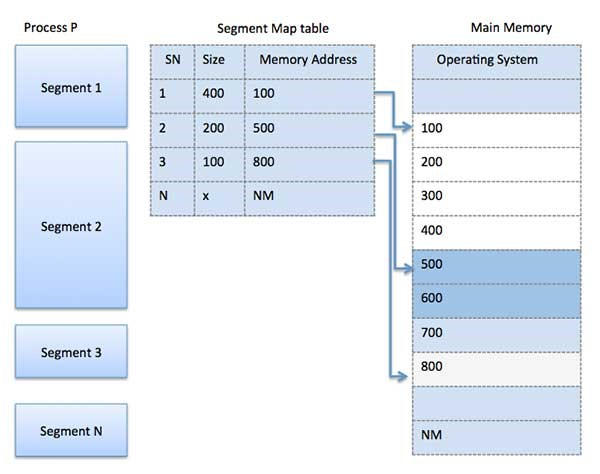
\includegraphics[width=1\textwidth]{..figures/segmentation.jpg}}
  \caption{Contoh segmentation}
  \label{segmentation}
  \end{figure}

\section{Pengertian Segmentation}
ini adalah contoh segmentation \ref{segmentation}
Segmentasi adalah teknik manajemen memori di mana setiap pekerjaan dibagi menjadi beberapa segmen dengan ukuran yang berbeda, satu untuk setiap modul yang berisi potongan-potongan yang melakukan fungsi terkait. Setiap segmen sebenarnya merupakan ruang alamat logis yang berbeda dari program.

%\chapter[Internet]
%{Definisi\\ Internet}
%\input{section/1internet.tex}

%\chapter[Web]
%{Definisi\\ Web}
%\input{section/1web.tex}

%\chapter[Backend]
%{Definisi\\ Backend}
%\input{section/1Backend.tex}

%\chapter[Frontend]
%{Definisi\\ Frontend}
%\input{section/1Frontend.tex}

% contoh aplikasi web service
% web service
% protokol
% port

% HTTP
% URL
% POST
% GET


\bibliographystyle{IEEEtran}
\bibliography{references, segmentation}

\printindex

\end{document}
